\section{Activity \# 1 - First Steps}

\frameboxbegin{Summary of the Activity}
Total duration: 30 minutes
The required equipment for this activities should be:
\begin{itemize}
\item 1 robot POB;
\item 1 computer with Risbee software installed;
\item 1 mini-USB cable;
\item 2 objects/targets
\item the booklet ``Quick Start Risbee''.
\end{itemize}
\frameboxend

\frameboxbegin{Motion - 5 minutes}
\begin{description}
\item[Objective:] To be able to move forward the robot.
\item[I am learning:] \hfill \\ \vspace{-4ex}
  \begin{itemize}
  \item To order the icons in order to make a simple program;
  \item To move the robot forward;
  \item The concept of trajectory.
  \end{itemize}
\end{description}
\frameboxend

\frameboxbegin{Stroll - 10 minutes}
\begin{flushleft}
\begin{description}
\item[Objectives:] To move the robot until a landmark ``A'' and stop it for few seconds. Then, move the robot forward to a landmark ``B'' and stop it for few seconds again. See Fig.\,\ref{fig:s} for details.
\begin{minipage}[c]{\textwidth}
\centering
\tikzstyle{target}=[circle,thick,minimum size=2cm,draw=blue!80,fill=blue!20]
\vspace{1ex}
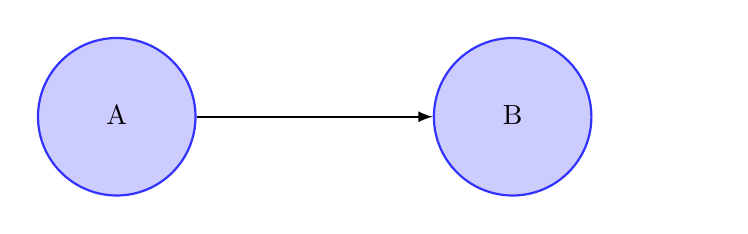
\begin{tikzpicture}[>=latex,text height=1.5ex,text depth=0.25ex]
  \matrix[row sep=1.5cm,column sep=1.5cm] {
    \node (A) [target] {A}; &
    &
    \node (B) [target] {B}; &
    \\
  };
  \path[->]
  (A) edge[thick] (B);
\end{tikzpicture}
\captionof{figure}{Landmarks positioning.}\label{fig:s}
\end{minipage}
\item[I am learning:] \hfill \\ \vspace{-1ex}
  \begin{itemize}
  \item To discover some additional icons;
  \item To move the robot forward until a given landmark;
  \item To stop the robot;
  \item The concept of trajectory.
  \end{itemize}
\end{description}
\end{flushleft}
\frameboxend

\frameboxbegin{Obstacle Avoidance - 10 minutes}
\begin{flushleft}
\begin{description}
\item[Objectives:] To reach the landmark ``B'' from landmark ``A'' by moving the robot only in straight line and turning at $90^{\circ}$. The two landmarks should be placed as depicted in Fig.\,\ref{fig:oa}. The player can choose in which side to start moving the robot. 
\begin{minipage}[c]{\textwidth}
\centering
\tikzstyle{target}=[circle,thick,minimum size=2cm,draw=blue!80,fill=blue!20]
\vspace{1ex}
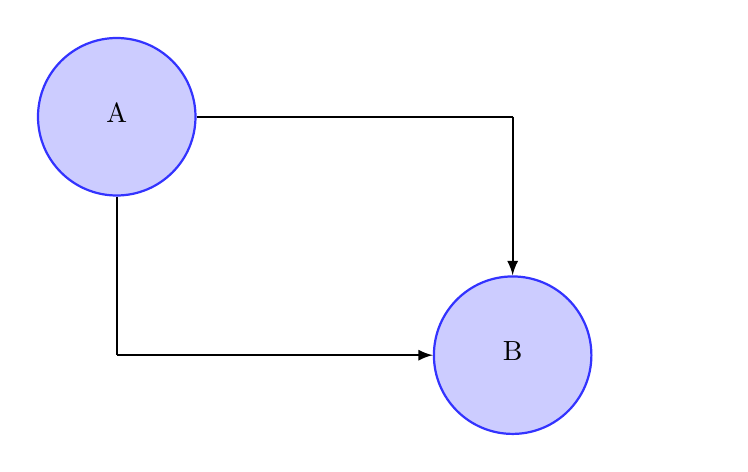
\begin{tikzpicture}[>=latex,text height=1.2ex,text depth=0.25ex]
  \matrix[row sep=.5cm,column sep=1.5cm] {
    \node (A) [target] {A}; &
    &
    \node (abtop) {};&
    \\
    & 
    & 
    &
    \\
    \node (abdown) {};&
    &
    \node (B) [target] {B}; &
    \\
  };
  \path[draw]
  (A) edge[thick] (abtop.center)
  (A) edge[thick] (abdown.center);
  \path[->]
  (abtop.center) edge[thick] (B)
  (abdown.center) edge[thick] (B);
\end{tikzpicture}
\captionof{figure}{Landmarks positioning.}\label{fig:oa}
\end{minipage}
\item[I am learning:] \hfill \\ \vspace{-1ex}
  \begin{itemize}
  \item The concept of angle.
  \end{itemize}
\end{description}
\end{flushleft}
\frameboxend

\frameboxbegin{Race - 5 minutes}
\begin{flushleft}
\begin{description}
\item[Objective:] To make a race between two robots. Move the position of the landmark ``B'' which will have to be reached by the players.
\item[I am learning:] \hfill \\ \vspace{-1ex}
  \begin{itemize}
  \item To discover some additional icons;
  \item To control the speed of the engines;
  \item To challenge other players.
  \end{itemize}
\end{description}
\end{flushleft}
\frameboxend
